\documentclass[10pt, aspectratio=169]{beamer}
\usepackage[utf8]{inputenc}
\usepackage{tikz}
\usetikzlibrary{shapes.geometric, arrows, shadows, positioning, patterns}

% --- Modern Tech Palette ---
\definecolor{deepnavy}{RGB}{10, 25, 47}
\definecolor{neonblue}{RGB}{100, 255, 218}
\definecolor{neongreen}{RGB}{0, 255, 127}
\definecolor{silver}{RGB}{204, 214, 246}
\definecolor{darkgray}{RGB}{35, 35, 35}

\setbeamercolor{background canvas}{bg=deepnavy}
\setbeamercolor{title}{fg=neonblue}
\setbeamercolor{frametitle}{fg=neonblue}
\setbeamercolor{normal text}{fg=silver}
\setbeamertemplate{navigation symbols}{}

\begin{document}

% --- SLIDE 1: THE EFFICIENCY GAP ---
\begin{frame}
    \vspace{0.2cm}
    \begin{center}
        \textcolor{neonblue}{\Large \textbf{Is Your AI Model "Lazy"?}} \\
        \small \textit{Unlocking Edge Performance via Activation-Based Structural Pruning}
    \end{center}
    
    \begin{columns}[T]
        \begin{column}{0.5\textwidth}
            \vspace{0.4cm}
            \textbf{\small THE EFFICIENCY GAP} \\
            \vspace{0.2cm}
            Standard models are over-engineered. They carry "Dead Weight" that slows down inference. \\
            \vspace{0.5cm}
            \textbf{\small OUR APPROACH: THE "X-RAY" SCAN} \\
            \vspace{0.2cm}
            \begin{itemize}
                \item \small \textbf{Behavioral Analysis:} We don't just look at weights; we monitor real-time filter activity.
                \item \small \textbf{Sensitivity Mapping:} Identifying the vital "Signal" vs. the redundant "Noise."
                \item \small \textbf{Precision Cut:} Removing the neurons that stay dark during inference.
            \end{itemize}
        \end{column}
        
        \begin{column}{0.5\textwidth}
            \centering
            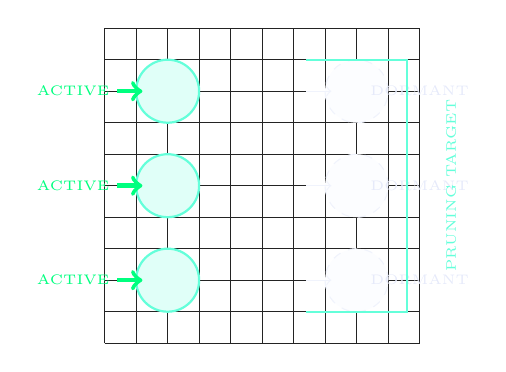
\begin{tikzpicture}[scale=0.8]
                % Grid Background for tech feel
                \draw[step=0.5, darkgray, thin] (-1,0) grid (4,5);
                
                % Active Nodes
                \foreach \y in {1,2.5,4} {
                    \node[circle, draw=neonblue, fill=neonblue!20, minimum size=0.8cm, thick] (a\y) at (0,\y) {};
                    \draw[neongreen, ultra thick, ->] (-0.8,\y) -- (-0.4,\y);
                    \node[text=neongreen] at (-1.5, \y) {\tiny ACTIVE};
                }
                
                % Dormant Nodes
                \foreach \y in {1,2.5,4} {
                    \node[circle, draw=silver!30, fill=silver!5, minimum size=0.8cm, dashed] (d\y) at (3,\y) {};
                    \draw[silver!30, thin, ->] (2.2,\y) -- (2.6,\y);
                    \node[text=silver!50] at (4, \y) {\tiny DORMANT};
                }
                
                % Target Bracket
                \draw[neonblue, thick] (2.2, 0.5) -- (3.8, 0.5) -- (3.8, 4.5) -- (2.2, 4.5);
                \node[text=neonblue, rotate=90] at (4.5, 2.5) {\tiny PRUNING TARGET};
            \end{tikzpicture}
        \end{column}
    \end{columns}
\end{frame}

% --- SLIDE 2: HARDWARE-READY AI ---
\begin{frame}
    \vspace{0.2cm}
    \begin{center}
        \textcolor{neonblue}{\Large \textbf{From Research to Real-World Edge Deployment}} \\
        \small \textit{Physical Surgery for Sub-Millisecond Latency}
    \end{center}

    \begin{columns}[T]
        \begin{column}{0.5\textwidth}
            \centering
            \vspace{0.5cm}
            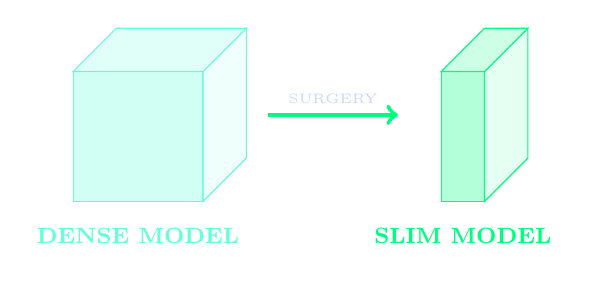
\begin{tikzpicture}[scale=0.55]
                % Original Fat Layer
                \draw[fill=neonblue!30, draw=neonblue] (0,0) -- (3,0) -- (3,3) -- (0,3) -- cycle;
                \draw[fill=neonblue!10, draw=neonblue] (3,0) -- (4,1) -- (4,4) -- (3,3) -- cycle;
                \draw[fill=neonblue!20, draw=neonblue] (0,3) -- (1,4) -- (4,4) -- (3,3) -- cycle;
                \node[text=neonblue] at (1.5, -0.8) {\footnotesize \textbf{DENSE MODEL}};
                
                % Scalpel Arrow
                \draw[->, ultra thick, neongreen] (4.5, 2) -- (7.5, 2) node[midway, above, text=silver] {\tiny SURGERY};
                
                % Pruned Slim Layer
                \begin{scope}[shift={(8.5,0)}]
                    \draw[fill=neongreen!30, draw=neongreen] (0,0) -- (1,0) -- (1,3) -- (0,3) -- cycle;
                    \draw[fill=neongreen!10, draw=neongreen] (1,0) -- (2,1) -- (2,4) -- (1,3) -- cycle;
                    \draw[fill=neongreen!20, draw=neongreen] (0,3) -- (1,4) -- (2,4) -- (1,3) -- cycle;
                    \node[text=neongreen] at (0.5, -0.8) {\footnotesize \textbf{SLIM MODEL}};
                \end{scope}
            \end{tikzpicture}
        \end{column}
        
        \begin{column}{0.5\textwidth}
            \vspace{0.4cm}
            \textbf{\small THE OUTCOME} \\
            \vspace{0.2cm}
            Structural pruning doesn't just "zero out" weights—it physically resizes the architecture. \\
            \vspace{0.4cm}
            \begin{itemize}
                \item \small \textbf{Speed:} 2x-3x faster inference on CPU/Mobile.
                \item \small \textbf{Efficiency:} 50\% reduction in FLOPs \& Energy.
                \item \small \textbf{Integrity:} SOTA accuracy with a fraction of the footprint.
            \end{itemize}
            \vspace{0.3cm}
            
\begin{tikzpicture}
                \node[draw=neongreen, fill=neongreen!10, rounded corners, inner sep=6pt, text=neongreen] at (0,0) {\textbf{\footnotesize \checkmark READY FOR PRODUCTION}};
            \end{tikzpicture}
        \end{column}
    \end{columns}
\end{frame}

\end{document}
